%%%%%%%%%%%%%%%%%%%%%%%%%%%%%%%%%%%%%%%%%%%%%%%%%%%%%%%%%%%%%%%%%%%%%%%%
% Plantilla TFG/TFM
% Escuela Politécnica Superior de la Universidad de Alicante
% Realizado por: Jose Manuel Requena Plens
% Contacto: info@jmrplens.com / Telegram:@jmrplens
%%%%%%%%%%%%%%%%%%%%%%%%%%%%%%%%%%%%%%%%%%%%%%%%%%%%%%%%%%%%%%%%%%%%%%%%
\clearpage

\thispagestyle{plain}
\chapter{Resultados}
\label{resultados}

  En esta sección se detallarán los resultados de cada una de las etapas del proyecto y los experimentos finales para realizar una discusión y un análisis comparativo entre ellos.

\section{Ejecución del Algoritmo Genético}

  En primer lugar analizaremos la optimización de los hiperparámetros del \glsentryshort{xgboost} gracias al algoritmo genético. En la figura \eqref{EvolucionHiperparametrosImage} se pueden visualizar la evolución de los hiperparámetros del mejor individuo en cada generación a través del transcurso de las iteraciones. Se puede observar cómo el mejor individuo de cada generación va variando los hiperparámetros probando distintos valores hasta converger aproximadamente en la iteración \textit{21}.

  \begin{figure}[h]
      \centering
      \includesvg[scale=0.35]{archivos/5.Resultados/GA/EvolucionHiperparametros}
      \caption{Evolución de hiperparámetros a lo largo de las iteraciones.}
      \label{EvolucionHiperparametrosImage}
   \end{figure}



  Como el mejor individuo obtenido en la ejecución de un algoritmo genético depende en gran medida de la inicialización de la población, se han realizado 50 ejecuciones del algoritmo con sus distintas inicializaciones. Nótese que un individuo del algoritmo genético está formado por 3 variables que representan los hiperparámetros. Así, el mejor individuo obtenido, de entre todas las ejecuciones, se puede observar en la tabla \eqref{BestGASolutionTable}.

  \begin{table}[h]
      \small
      \centering
          \begin{tabular}{ |c|c| } 
              \hline
              \textbf{Hiperparámetro} & \textbf{Valor}\\
              \hline
                  Profundidad Máxima & 1 \\
                  Peso mínimo de los hijos & 0.01 \\ 
                  ETA & 0.049 \\ 
              \hline

          \end{tabular}
      \caption{Mejores parámetros de XGBoost tras aplicar el algoritmo genético.}
      \label{BestGASolutionTable}
  \end{table}


\section{Ejecución del modelo XGBoost}

  Una vez obtenidos los principales hiperparámetros óptimos, es el turno de aplicar el algoritmo \glsentryshort{xgboost} para calcular los pesos de las variables. En la figura \eqref{FeatureWeightsImage} se puede observar un diagrama de barras en el que las características \textit{tipo de persona}, \textit{tipo de carretera} y \textit{sexo} son las que más han influido a la hora de entrenar el modelo \glsentryshort{xgboost}, obteniendo unos pesos de \textit{0.177}, \textit{0.127} y \textit{0.111} respectivamente. Los resultados obtenidos por este algoritmo se han obtenido estableciendo una semilla sobre la división de los datos de entrenamiento y test, para poder reproducir los valores de los pesos en experimentos posteriores. Se pueden consultar los pesos calculados de todas las características en la tabla \eqref{PesosFinalesCaracteristicas}, en la que los pesos de las categorías padres es la suma de cada una de las características hijas.


  \begin{figure}[h]
      \centering
      \includesvg[scale = 0.55]{archivos/5.Resultados/XGBoost/FeatureWeights}
      \caption{Pesos asignados por XGboost a las características.}
      \label{FeatureWeightsImage}
   \end{figure}


  \begin{table}[H]
    \small
    \centering
    \begin{tabular}{ |c|c|c|c| }
         \hline
         \textbf{Categoría} & \textbf{Peso Categoría} & \textbf{Característica} & \textbf{Peso Característica}\\

         \hline
         \multirow{4}{*}{Accidente}   & \multirow{4}{*}{0.299}        & Coordenada X          & 0.071\\
                                      &                               & Coordenada Y          & 0.066\\
                                      &                               & Hora                  & 0.055\\
                                      &                               & Vehículos implicados  & 0.051\\
                                      &                               & Tipo de accidente     & 0.057\\
         \hline

    \end{tabular}
  \end{table}
  \begin{table}[H]
    \small
    \centering                            
    \begin{tabular}{ |c|c|c|c| }
         \hline
         \textbf{Categoría} & \textbf{Peso Categoría} & \textbf{Característica} & \textbf{Peso Característica}\\
         \hline

         \multirow{2}{*}{Carretera}   & \multirow{2}{*}{0.187}        & Distrito              & 0.059\\      
                                      &                               & Tipo carretera        & 0.127\\

         \hline
         \multirow{1}{*}{Ambiente}    & \multirow{1}{*}{0.050}        & Estado meteorológico  & 0.050\\

         \hline
         \multirow{1}{*}{Vehículo}    & \multirow{1}{*}{0.070}        & Tipo de vehículo      & 0.070\\


         \hline
         \multirow{4}{*}{Conductor}   & \multirow{4}{*}{0.394}        & Tipo Persona          & 0.177\\
                                      &                               & Sexo                  & 0.111\\
                                      &                               & Rango Edad            & 0.050\\
                                      &                               & Positivo              & 0.056\\
         \hline

    \end{tabular}

    \caption{Cálculo de pesos de características y categorías mediante XGBoost (los valores se han redondeado en base a tres decimales).}
    \label{PesosFinalesCaracteristicas}
  \end{table}

\section{Matrices}

  En esta sección se mostrará el proceso que sigue una observación del dataset original tipificada hasta llegar a una matriz de características \eqref{ProcesoMatriz}. En primer lugar, los valores de la muestra original \eqref{ProcesoMatriz:MuestraTipificada} se normalizan según el criterio \glsentrylong{zsn} para pasar a ser una observación cuyos valores estan acotados en un rango en función de la distribución normal de cada característica en el dataset \eqref{ProcesoMatriz:MuestraNormalizada}. Ahora se suman los pesos de las características hijas para obtener el peso de las categorías padre. El siguiente paso será posicionar cada uno de los valores de la muestra la matriz, de acuerdo a los índices calculados en el paso anterior. Estas matrices sirven como entrada a las redes neuronales convolucionales \eqref{ProcesoMatriz:Array}.

    \begin{figure}[H]
        \scriptsize
        \centering
        \renewcommand{\arraystretch}{1.4}

        \captionsetup{singlelinecheck = false, format= hang, justification=raggedright, font=footnotesize, labelsep=space}

        \begin{subtable}{.4\textwidth}
          \centering
          \csvautotabular{archivos/5.Resultados/Matrices/fatal_original.csv}

          \captionsetup{singlelinecheck = false, format= hang, justification=centering, font=footnotesize, labelsep=space}
          
          \caption{Muestra de accidente tipificada.}
          \label{ProcesoMatriz:MuestraTipificada}
        \end{subtable}
        \hspace{20mm}
        \renewcommand{\arraystretch}{1.4}
        \begin{subtable}{.4\textwidth}
          \hspace{5mm}
          \csvautotabular{archivos/5.Resultados/Matrices/fatal_normalized.csv}
          \caption{Muestra de accidente normalizada.}
          \label{ProcesoMatriz:MuestraNormalizada}
        \end{subtable}
    \end{figure}%
    \begin{figure}[H]\ContinuedFloat
        \scriptsize
        \centering
        \vskip\baselineskip
        \begin{subtable}{.4\textwidth}
          \centering
          \renewcommand{\arraystretch}{1.5}

          \csvreader[
            tabular = |c|c|c|c|c|,
            table head = \hline,
            table foot = \hline
            ]{archivos/5.Resultados/Matrices/fatal_matrix.csv}%
            {0=\cero, 1=\one, 2=\two, 3=\three, 4=\four}{%
            \cero & \one & \two & \three &  \four
          }
          \captionsetup{singlelinecheck = false, format= hang, justification=centering, font=footnotesize, labelsep=space}
          \caption{Características.}
          \label{ProcesoMatriz:Array}
        \end{subtable}
        \hspace{5em}
        \begin{subfigure}{0.4\textwidth}
          \centering
          \includesvg[scale=0.5]{archivos/5.Resultados/Matrices/accidente_fatal}
          \captionsetup{singlelinecheck = false, format= hang, justification=centering, font=footnotesize, labelsep=space}
          \caption{Imagen de las características.}
          \label{ProcesoMatriz:VisualizacionDeMatriz}
        \end{subfigure}
      \caption{Proceso que sigue una muestra del conjunto de datos tipificada hasta llegar a una matriz (a $\rightarrow$ b $\rightarrow$ c $\rightarrow$ d).}
      \label{ProcesoMatriz}
      \end{figure}



  A modo de ejemplo se muestra en la figura \eqref{TresClasesAccidentesMatrices} un accidente de cada clase transformados a su matriz correspondiente.

  \begin{figure}[H]
      \centering
      \scriptsize
      \begin{subtable}{.4\textwidth}
        \centering
        \renewcommand{\arraystretch}{1.5}

        \csvreader[
          tabular = |c|c|c|c|c|,
          table head = \hline,
          table foot = \hline
          ]{archivos/5.Resultados/Matrices/slight_matrix.csv}%
          {0=\cero, 1=\one, 2=\two, 3=\three, 4=\four}{%
          \cero & \one & \two & \three &  \four
        }
        \caption{Características leves.}
        \label{ProcesoMatriz:Array}
      \end{subtable}
      \hspace{5em}
      \begin{subfigure}[b]{.4\textwidth}
        \centering
        \includesvg[scale=0.4]{archivos/5.Resultados/Matrices/accidente_leve}
        \caption{Accidente leve.}
        \label{TresClasesAccidentesMatrices:AccidenteLeveImage}
      \end{subfigure}
      \vskip\baselineskip
      \begin{subtable}{.4\textwidth}
        \centering
        \renewcommand{\arraystretch}{1.5}

        \csvreader[
          tabular = |c|c|c|c|c|,
          table head = \hline,
          table foot = \hline
          ]{archivos/5.Resultados/Matrices/serious_matrix.csv}%
          {0=\cero, 1=\one, 2=\two, 3=\three, 4=\four}{%
          \cero & \one & \two & \three &  \four
        }
        \caption{Características severas.}
        \label{ProcesoMatriz:Array}
      \end{subtable}
      \hspace{5em}
      \begin{subfigure}[b]{.4\textwidth}
        \centering
        \includesvg[scale=0.4]{archivos/5.Resultados/Matrices/accidente_severo}
        \caption{Accidente severo.}
        \label{TresClasesAccidentesMatrices:AccidenteSeveroImage}
      \end{subfigure}
      \vskip\baselineskip
      \begin{subtable}{.4\textwidth}
        \centering
        \renewcommand{\arraystretch}{1.5}

        \csvreader[
          tabular = |c|c|c|c|c|,
          table head = \hline,
          table foot = \hline
          ]{archivos/5.Resultados/Matrices/fatal_matrix.csv}%
          {0=\cero, 1=\one, 2=\two, 3=\three, 4=\four}{%
          \cero & \one & \two & \three &  \four
        }
        \caption{Características fatales.}
        \label{ProcesoMatriz:Array}
      \end{subtable}
      \hspace{5em}
      \begin{subfigure}[b]{0.4\textwidth}
        \centering
        \includesvg[scale=0.4]{archivos/5.Resultados/Matrices/accidente_fatal}
        \caption{Accidente fatal.}
        \label{TresClasesAccidentesMatrices:AccidenteFatalImage}
      \end{subfigure}


    \caption{Tres matrices de accidentes representadas como imágenes.}
    \label{TresClasesAccidentesMatrices}
  \end{figure}

  Una vez convertidos los accidentes en matrices, estas actúan como entrada a las redes neuronales convolucionales.

%%%%%%%%%%%%%%%%%%%%%%%%%%%%%%%%%%%%%%%%%%%%%%%%%%%%%%%%%%%%%%%%%%%%%%%%%%%%%%%%%%%%%%%%%%%%%%%%%%%%%%%%%%%%%%%%%%%%%%%%%%%%%%%%%%%%%%%%%%%%%%%%%%%%%%%%%%%%%%%%%%%%%%%%%%%%%%%%%%%%%%%%%%%%%%%%%%%%%%%%%%%%%%%%%%%%%%%%%%%%%%%%%%%%%%%%%%%%%%%%%%%%%%%%%%%%%%%%%%%%%%%%%%%%%%%%%%%%%%%%%%%%%%%%%%%%%%%%%%%%%%%%%%%%%%%%%%%%%%%%%%%%%%%%%%%%%%%%%%%%%%%%%%%%%%%%%%%%%%%%%%%%%%%%%%%%%%%%%%%%%%%%%%%%%%%%%%%%%%%%%%%%%%%%%%%%%%%%%%%%%%%%%%%%%%%%%%%%%%%%%%%%%%%%%%%%%%%%%%%%%%%%%%%%%%%%%%%%%%%%%%%%%%%%%%%%%%%%%%%%%%%%%%%

\section{Entrenamiento de modelos convolucionales}


  En esta subsección se va a detallar todo lo relativo al modelo basado en redes neuronales convolucionales. Se estudiarán los siguientes elementos:

  \begin{enumerate}
    \item Rendimiento computacional
    \item Evolución de la función de pérdida
    \item Resultados de la predicción en base a métricas de clasificación, optimización y matrices de confusión
  \end{enumerate}


  \subsection{Tiempos de entrenamiento}


    En la figura \eqref{ClassificationReportCNN} se muestran los tiempos de entrenamiento transcurrido por ambas redes, donde se puede apreciar que la \glsentryshort{cnn1d} emplea más tiempo (\textit{287 seg}) que la \glsentryshort{cnn2d seg} (\textit{259} seg), debido a que los kernels son de menor tamaño, por lo que deberá convolucionar mayor número de veces respecto al kernel de mayor tamaño de la \glsentryshort{cnn2d}.

    \begin{figure}[h]
      \centering
      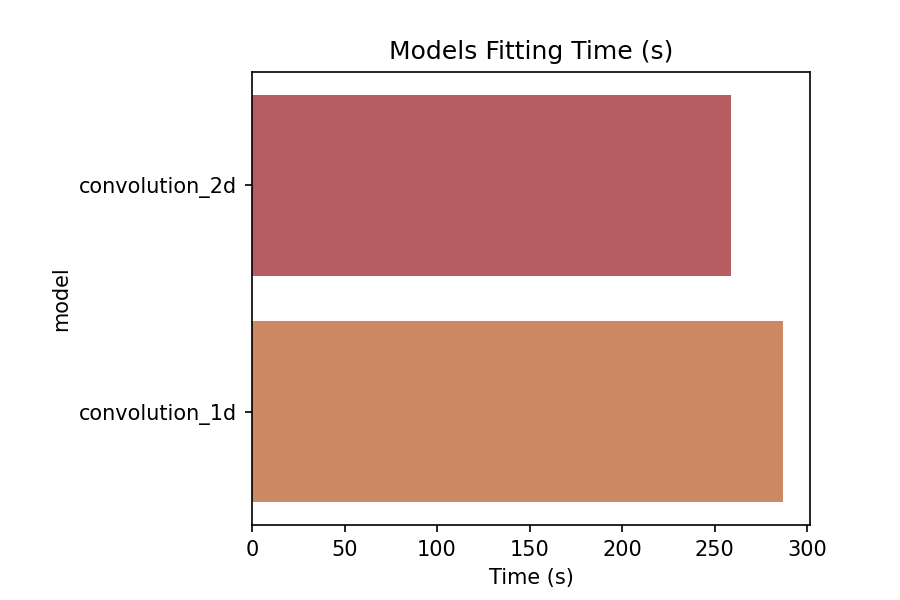
\includegraphics[width=8cm]{archivos/5.Resultados/only_cnns_times}
      \caption{Comparación de tiempo de entrenamiento entre las redes neuronales convolucionales.}
      \label{TiemposEntrenamientoCNNImage}
    \end{figure}



  \subsection{Gráficas de entrenamiento}


    En las figuras \eqref{F1ScoreEvolution:1D} y \eqref{F1ScoreEvolution:2D} se puede observar la evolución de la métrica definida a maximizar (Micro F1-score) a lo largo de las 100 épocas que se han ejecutado para las redes convolucionales. Visualizando la gráfica de la convolucional de una dimensión \eqref{F1ScoreEvolution:1D} se puede comprobar que el Micro F1-score de entrenamiento va aumentando ligeramente a lo largo de las épocas sufriendo altibajos a medida que el modelo es entrenado, partiendo inicialmente desde un valor de entrenamiento menor a \textit{0.58} y llegando hasta \textit{0.68}. Observamos que los datos de validación sufren continuamente variaciones sin llegar a obtener una tendencia estable. Esto es debido a que, con la complejidad del problema, estos datos se asignan casi aleatoriamente entre las épocas.\\


    \begin{figure}[H]
        \centering
        \includesvg[scale=0.25]{archivos/5.Resultados/CNN/1D/F1Score1D}
        \caption{Evolución de Micro F1-score sobre el conjunto de entrenamiento y validación CNN-1D.}
        \label{F1ScoreEvolution:1D}
    \end{figure}
    \begin{figure}[H]
        \centering
        \includesvg[scale=0.25]{archivos/5.Resultados/CNN/2D/F1Score2D}
        \caption{Evolución de Micro F1-score sobre el conjunto de entrenamiento y validación CNN-2D.}
        \label{F1ScoreEvolution:2D}
    \end{figure}


    En la figura \eqref{F1ScoreEvolution:2D} se puede apreciar la gráfica de entrenamiento y validación de la red convolucional de dos dimensiones. Observando que la tendencia de la función de pérdida sobre el conjunto de datos de entrenamiento es más estable respecto a la convolucional de una dimensión. Se aprecia cómo la red en la primera época comienza con un Micro F1-score de \textit {0.62} hasta llegar a \textit{0.78} en la época \textit{100}, por lo que se puede deducir que esta red consigue un mejor rendimiento sobre el conjunto de entrenamiento respecto a la red convolucional de una dimensión. Respecto a los datos de validación nos encontramos frente al mismo caso que la anterior figura, en cada epoch muchos de los datos son clasificados aleatoriamente debido a la complejidad del problema.

  \subsection{Métricas de clasificación}

    En la tabla \eqref{ClassificationReportCNN} se detallan las métricas resultantes de la clasificación de las redes para sus conjuntos de entrenamiento y test. Se observa que para el conjunto de entrenamiento el modelo \glsentryshort{cnn1d} \eqref{ClassificationReportCNN:TrainCNN1D} obtiene un mejor F1-score sobre la clasificación de todas las clases de accidentes respecto a la red \glsentryshort{cnn2d} \eqref{ClassificationReportCNN:TrainCNN2D}. Sin embargo, si se analizan las métricas de los datos de test, el modelo que mejor F1-score presenta para los accidentes leves y severos es la \glsentryshort{cnn2d} \eqref{ClassificationReportCNN:TestCNN1D}, con \textit{0.949} y \textit{0.149} respectivamente, mientras que la \glsentryshort{cnn1d} obtiene una mejor clasificación sobre los fatales \eqref{ClassificationReportCNN:TestCNN2D} \textit{0.004}.

    \begin{figure}[H]
        \scriptsize
        %\captionsetup{singlelinecheck = false, format= hang, justification=raggedright, font=footnotesize, labelsep=space}
        \renewcommand{\arraystretch}{1.1}
        \begin{subtable}{.5\textwidth}        
          \csvautotabular{archivos/5.Resultados/CNN/1D/1DClassificationReportTrain.csv}
          \caption{Métricas de entrenamiento CNN-1D.}
          \label{ClassificationReportCNN:TrainCNN1D}
        \end{subtable}
        \hspace{1em}
        \begin{subtable}{.5\textwidth}
          \centering
          \csvautotabular{archivos/5.Resultados/CNN/2D/2DClassificationReportTrain.csv}
          \caption{Métricas de entrenamiento CNN-2D.}
          \label{ClassificationReportCNN:TrainCNN2D}
        \end{subtable}
        \vspace*{2mm}
        \begin{subtable}{.5\textwidth}     
          \csvautotabular{archivos/5.Resultados/CNN/1D/1DClassificationReportTest.csv}
          \caption{Métricas de test CNN-1D.}
          \label{ClassificationReportCNN:TestCNN1D}
        \end{subtable}
        \hspace{.75em}
        \begin{subtable}{.5\textwidth}     
          \centering
          \csvautotabular{archivos/5.Resultados/CNN/2D/2DClassificationReportTest.csv}
          \caption{Métricas de test CNN-2D.}
          \label{ClassificationReportCNN:TestCNN2D}
        \end{subtable}
        \caption{Métricas de clasificación para las redes neuronales convolucionales.}
        \label{ClassificationReportCNN}
    \end{figure}
  

  \subsection{Matrices de confusión}

    En la figura \eqref{ConfusionMatrixCNNImages} se muestran las matrices de confusión para los conjuntos de entrenamiento y test de ambos modelos, donde se pueden analizar las tendencias predictivas. Para los datos de entrenamiento de \glsentryshort{cnn2d} \eqref{ConfusionMatrixCNNImages:Train2D} se tiende a una mayor propensión a la hora de predecir las observaciones como accidentes leves respecto a la red \glsentryshort{cnn1d} \eqref{ConfusionMatrixCNNImages:Train1D}, dejando más muestras a clasificar del resto de clases por parte del segundo modelo. Esto provoca que la \glsentryshort{cnn1d} clasifique correctamente más accidentes serios y fatales. Para el conjunto de datos de test, la red \glsentryshort{cnn2d} \eqref{ConfusionMatrixCNNImages:Test2D} clasifica más observaciones como accidentes leves respecto al modelo \glsentryshort{cnn1d} \eqref{ConfusionMatrixCNNImages:Test1D}, prediciendo un menor número de accidentes serios pero con una mayor confianza.

    \begin{figure}[H]
      \centering
      \begin{subfigure}{0.4\textwidth}
          \includesvg[scale=0.35]{archivos/5.Resultados/CNN/1D/1DConfusionMatrixTrain}
          \caption{Entrenamiento CNN-1D.}
          \label{ConfusionMatrixCNNImages:Train1D}
      \end{subfigure}
      \hspace{1mm}
      \begin{subfigure}{0.4\textwidth}
          \includesvg[scale=0.35]{archivos/5.Resultados/CNN/2D/2DConfusionMatrixTrain}
          \caption{Entrenamiento CNN-2D.} 
          \label{ConfusionMatrixCNNImages:Train2D}
      \end{subfigure}
      \vspace*{2mm}
      \begin{subfigure}{0.4\textwidth}
          \includesvg[scale=0.35]{archivos/5.Resultados/CNN/1D/1DConfusionMatrixTest}
          \caption{Test CNN-1D.}
          \label{ConfusionMatrixCNNImages:Test1D}
      \end{subfigure}
      \hspace{1em}
      % Añadir el espacio deseado, si se deja la linea en blanco la siguiente subfigura ira en una nueva linea
      \begin{subfigure}{0.4\textwidth}
          \includesvg[scale=0.35]{archivos/5.Resultados/CNN/2D/2DConfusionMatrixTest}
          \caption{Test CNN-2D.} 
          \label{ConfusionMatrixCNNImages:Test2D}
      \end{subfigure}
      \caption{Matrices de confusión para las redes neuronales convolucionales.}
      \label{ConfusionMatrixCNNImages}
    \end{figure}

\clearpage

  \subsection{Gráficas de clasificación}

    En la figura \eqref{ResultsCNNImage} se muestra una representación visual, en forma de diagrama de barras, las métricas de clasificación para el conjunto de entrenamiento de ambos modelos \eqref{ResultsCNNImage:Train} al igual que para el conjunto de validación \eqref{ResultsCNNImage:Test}.

    \begin{figure}[H]
      \hspace{-2em}
      \begin{subfigure}{0.4\textwidth}        
        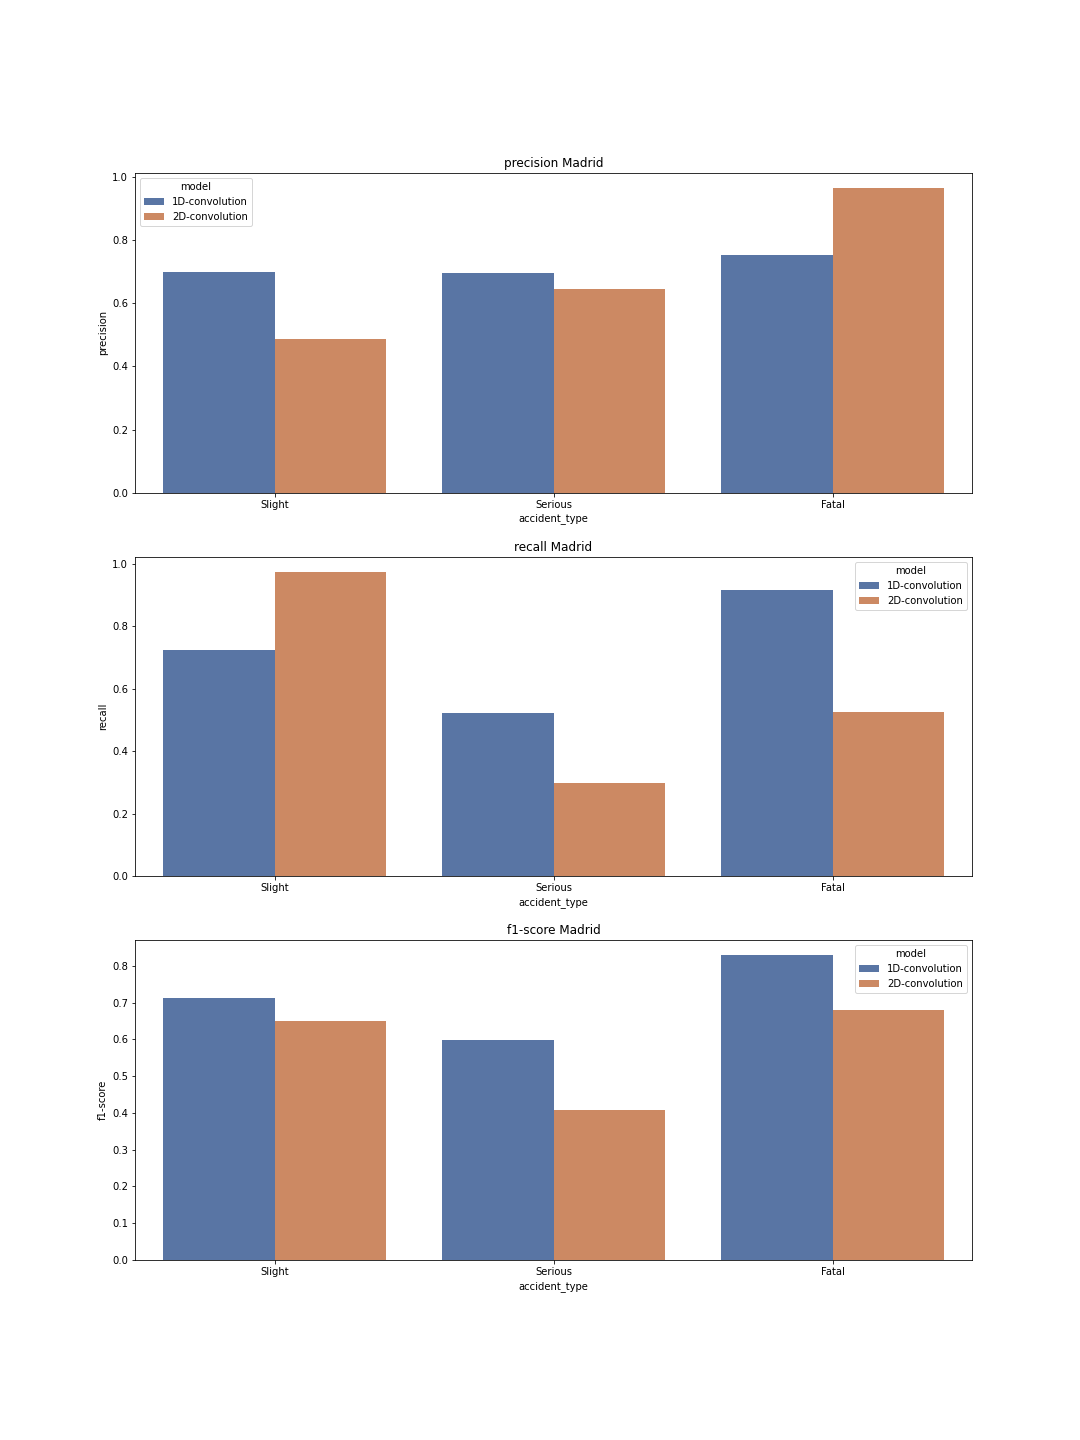
\includegraphics[width=9cm]{archivos/5.Resultados/ComparativaCNNTrain}
        \captionsetup{singlelinecheck = false, justification=centering, font=footnotesize}
        \caption{Entrenamiento.}
        \label{ResultsCNNImage:Train}
      \end{subfigure}
      \hspace{8mm}
      \begin{subfigure}{0.4\textwidth}        
        \centering
        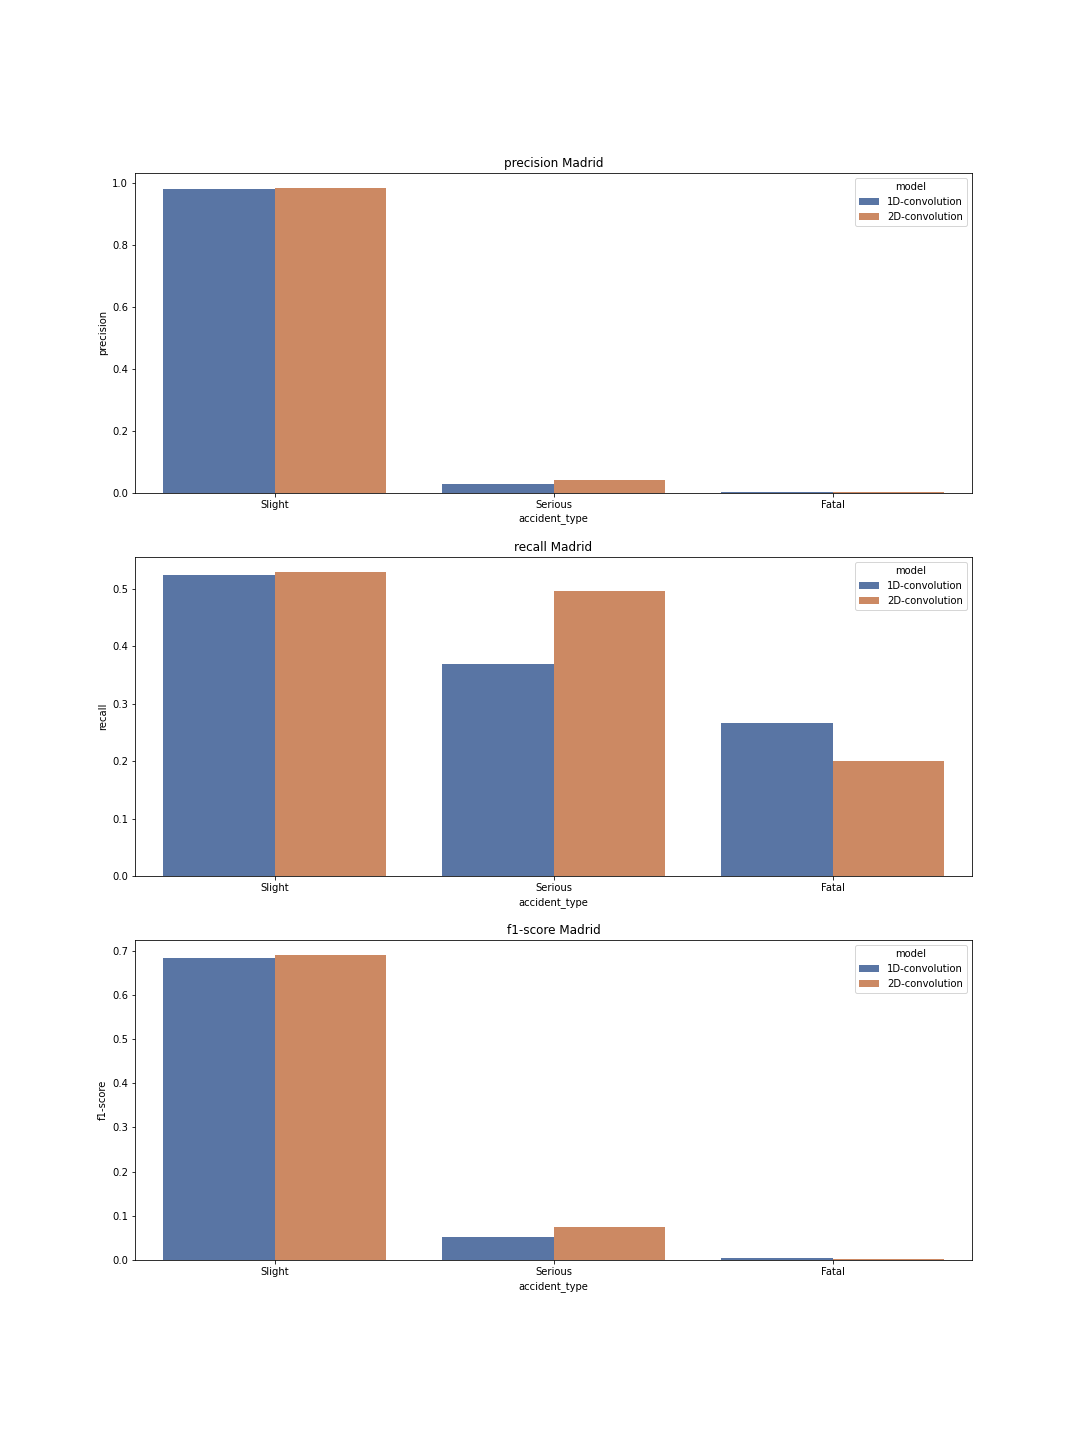
\includegraphics[width=9cm]{archivos/5.Resultados/ComparativaCNNTest}
        \caption{Test.}
        \label{ResultsCNNImage:Test}
      \end{subfigure}
      \caption{Comparativa de las métricas de las predicciones sobre el conjunto de entrenamiento y test de los modelos.}
      \label{ResultsCNNImage}
    \end{figure}




%%%%%%%%%%%%%%%%%%%%%%%%%%%%%%%%%%%%%%%%%%%%%%%%%%%%%%%%%%%%%%%%%%%%%%%%%%%%%%%%%%%%%%%%%%%%%%%%%%%%%%%%%%%%%%%%%%%%%%%%%%%%%%%%%%%%%%%%%%%%%%%%%%%%%%%%%%%%%%%%%%%%%%%%%%%%%%%%%%%%%%%%%%%%%%%%%%%%%%%%%%%%%%%%%%%%%%%%%%%%%%%%%%%%%%%%%%%%%%%%%%%%%%%%%%%%%%%%%%%%%%%%%%%%%%%%%%%%%%%%%%%%%%%%%%%%%%%%%%%%%%%%%%%%%%%%%%%%%%%%%%%%%%%%%%%%%%%%%%%%%%%%%%%%%%%%%%%%%%%%%%%%%%%%%%%%%%%%%%%%%%%%%%%%%%%%%%%%%%%%%%%%%%%%%%%%%%%%%%%%%%%%%%%%%%%%%%%%%%%%%%%%%%%%%%%%%%%%%%%%%%%%%%%%%%%%%%%%%%%%%%%%%%%%%%%%%%%%%%%%%%%%%%%


\section{Comparativa de modelos}


  Una vez obtenidos los resultados de los modelos vamos a efectuar una comparativa de las redes neuronales convolucionales. 

  \subsection{Entrenamiento}

  Lo primero es analizar los tiempos de entrenamiento, métricas de clasificación y matrices de confusión sobre el conjunto de datos de entrenamiento con respecto al resto de modelos  \glsentryshort{gnb}, \glsentryshort{knn} y \glsentryshort{svc}. Las métricas de clasificación para la predicción de los modelos sobre este conjunto no son concluyentes, ya que únicamente es útil para hacerse a la idea de cómo han evaluado los modelos las observaciones. Unos resultados prometedores sobre este conjunto no implican un buen rendimiento, ya que si se predice a la perfección el conjunto de entrenamiento es síntoma de que el modelo está sobreentrenado y, como consecuencia, conllevará una pobre generalización sobre el conjunto de validación. En esta sección se analizarán los resultados sobre el conjunto de entrenamiento para mostrar a modo orientativo cómo han entrenado los modelos.

  \subsubsection{Comparativa de tiempos de entrenamiento}

    En la figura \eqref{TiemposEntrenamientoImage} se comparan los tiempos de entrenamiento de cuatro modelos. Hay que recalcar que el método \glsentryshort{knn}, al proyectar las muestras de entrenamiento en un espacio n-dimensional, no conlleva un entrenamiento como tal. Observando la gráfica se puede apreciar que el modelo que más tiempo de entrenamiento emplea es el \glsentryshort{svc} con \textit{593} segundos, seguido de las redes convolucionales de una y dos dimensiones con \textit{287} y \textit{259} segundos respectivamente y, por último, el clasificador \glsentryshort{gnb}, que debido a su naturaleza es el que menos tiempo emplea en entrenar con \textit{0.02} segundos.

    \begin{figure}[h]
      \centering
      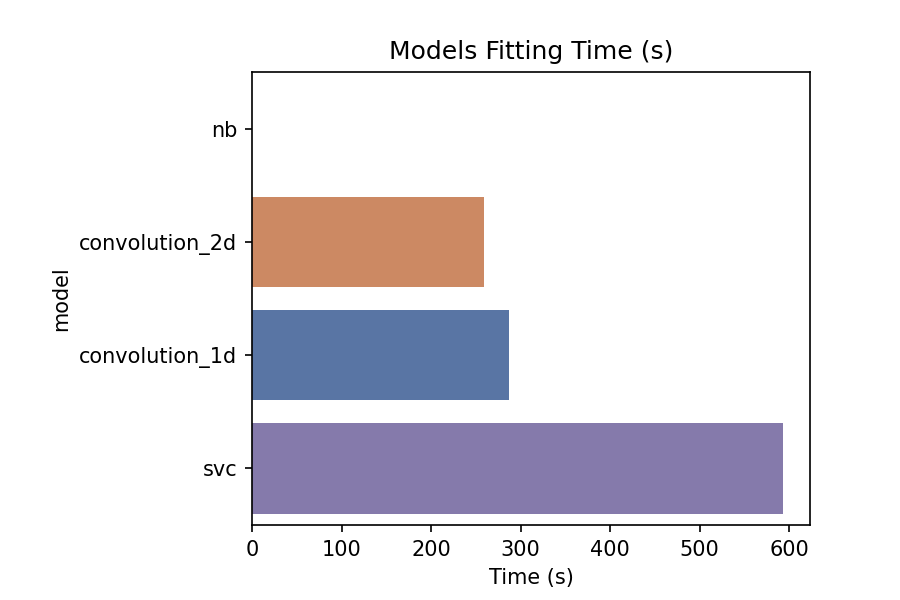
\includegraphics[width=8cm]{archivos/5.Resultados/TiemposEntrenamiento}
      \caption{Comparación entre los tiempos de entrenamiento de los modelos.}
      \label{TiemposEntrenamientoImage}
    \end{figure}


  \subsubsection{Comparativa de métricas de clasificación}

    En la figura \eqref{TrainClassificationReport} se muestra la comparativa de las métricas de clasificación resultantes de predecir los datos de entrenamiento con los que han aprendido los modelos, útil para comprender las tendencias de aprendizaje de cada modelo. Como se puede observar, el modelo que mejores métricas de entrenamiento ofrece basándonos en el F1-score es el \glsentryshort{svc} \eqref{TrainClassificationReport:SVC}, que consigue un valor medio de \textit{0.841}. En segundo y tercer lugar, nos encontramos con dos modelos que, dependiendo de la clase a predecir, se intercalan en rendimiento, éstos son la red neuronal convolucional de una dimensión \eqref{TrainClassificationReport:CNN1D} y \glsentryshort{knn} \eqref{TrainClassificationReport:KNN}, que obtienen una media F1-score de \textit {0.721} y \textit {0.724} respectivamente. El cuarto lugar se posiciona la red neuronal convolucional de dos dimensiones \eqref{TrainClassificationReport:CNN2D}, consiguiendo un F1-score medio de \textit{0.599}, no llegando a superar en ninguna clase el rendimiento de las anteriores. Por último, el modelo que peor resultados ofrece es el \textit{Gaussian Naive Bayes} \eqref{TrainClassificationReport:GNB}, que obtiene los valores más bajos de los cinco modelos entrenados con un valor medio F1-score de \textit{0.432}.

    \begin{table}[H]
        \scriptsize
        %\captionsetup{singlelinecheck = false, format= hang, justification=raggedright, font=footnotesize, labelsep=space}
        \renewcommand{\arraystretch}{1.1}
        \begin{subtable}{.5\textwidth}        
          \csvautotabular{archivos/5.Resultados/CNN/1D/1DClassificationReportTrain.csv}
          \caption{CNN-1D.}
          \label{TrainClassificationReport:CNN1D}
        \end{subtable}
        \hspace{1em}
        \begin{subtable}{.5\textwidth}
          \csvautotabular{archivos/5.Resultados/NB/NBClassificationReportTrain.csv}
          \caption{GNB.}
          \label{TrainClassificationReport:GNB}
        \end{subtable}
        \vspace*{2mm}
        \begin{subtable}{.5\textwidth}  
          \centering
          \csvautotabular{archivos/5.Resultados/SVC/SVCClassificationReportTrain.csv}
          \caption{SVC.}
          \label{TrainClassificationReport:SVC}
        \end{subtable}
        \hspace{1em}
        \begin{subtable}{.5\textwidth}
          \csvautotabular{archivos/5.Resultados/KNN/KNNClassificationReportTrain.csv}
          \caption{KNN.}
          \label{TrainClassificationReport:KNN}
        \end{subtable}
        \vspace*{2mm}
        %\captionsetup{justification=centering}
        \begin{subtable}{1\textwidth}
          \centering
          \csvautotabular{archivos/5.Resultados/CNN/2D/2DClassificationReportTrain.csv}
          \caption{CNN-2D.}
          \label{TrainClassificationReport:CNN2D}
        \end{subtable}
        \caption{Métricas clasificación para el conjunto de entrenamiento.}
        \label{TrainClassificationReport}
    \end{table}

\clearpage

  \subsubsection{Comparativa de matrices de confusión}

    En este apartado analizaremos las matrices de confusión de los experimentos con los datos de entrenamiento. A simple vista se observa que \glsentryshort{gnb} \eqref{ConfusionMatrixTrainImages:GNB} tiende a predecir un gran número de muestras como accidentes fatales, lo que significa que debido a la simplicidad de este modelo no se consiguen predecir el resto de accidentes correctamente. Por otro lado, los modelos que mayor número de muestras de entrenamiento consiguen clasificar correctamente son el \glsentryshort{svc} \eqref{ConfusionMatrixTrainImages:SVC}, \glsentryshort{knn} \eqref{ConfusionMatrixTrainImages:KNN} y \glsentryshort{cnn1d} \eqref{ConfusionMatrixTrainImages:1D}.

    \begin{figure}[H]
        \centering
        \begin{subfigure}{0.4\textwidth}
            \includesvg[scale=0.35]{archivos/5.Resultados/CNN/1D/1DConfusionMatrixTrain}
            \caption{CNN-1D.}
            \label{ConfusionMatrixTrainImages:1D}
        \end{subfigure}
        \hspace{1mm}
        \begin{subfigure}{0.4\textwidth}
            \includesvg[scale=0.35]{archivos/5.Resultados/CNN/2D/2DConfusionMatrixTrain}
            \caption{CNN-2D.} 
            \label{ConfusionMatrixTrainImages:2D}
        \end{subfigure}
        \vspace*{0.1 mm}
        \begin{subfigure}{0.4\textwidth}
            \includesvg[scale=0.35]{archivos/5.Resultados/NB/NBConfusionMatrixTrain}
            \caption{GNB.}
            \label{ConfusionMatrixTrainImages:GNB}
        \end{subfigure}
        \hspace{1mm}
        \begin{subfigure}{0.4\textwidth}
            \includesvg[scale=0.35]{archivos/5.Resultados/KNN/KNNConfusionMatrixTrain}
            \caption{KNN.}
            \label{ConfusionMatrixTrainImages:KNN}
        \end{subfigure}
        \vspace*{0.1 mm}
        \begin{subfigure}{1\textwidth}
            \centering
            \includesvg[scale=0.35]{archivos/5.Resultados/SVC/SVCConfusionMatrixTrain}
            \caption{SVC.}
            \label{ConfusionMatrixTrainImages:SVC}
        \end{subfigure}
        \caption{Matrices de confusión de los modelos sobre el conjunto de entrenamiento.}
        \label{ConfusionMatrixTrainImages}
     \end{figure}


  \subsubsection{Comparativa entre modelos}

  En la figura \eqref{ResultsTrainImage} se muestra gráficamente el rendimiento de cada modelo sobre el conjunto de entrenamiento, las métricas utilizadas son la precisión, exhaustividad y el F1-score.

  \begin{figure}[H]
      \centering
      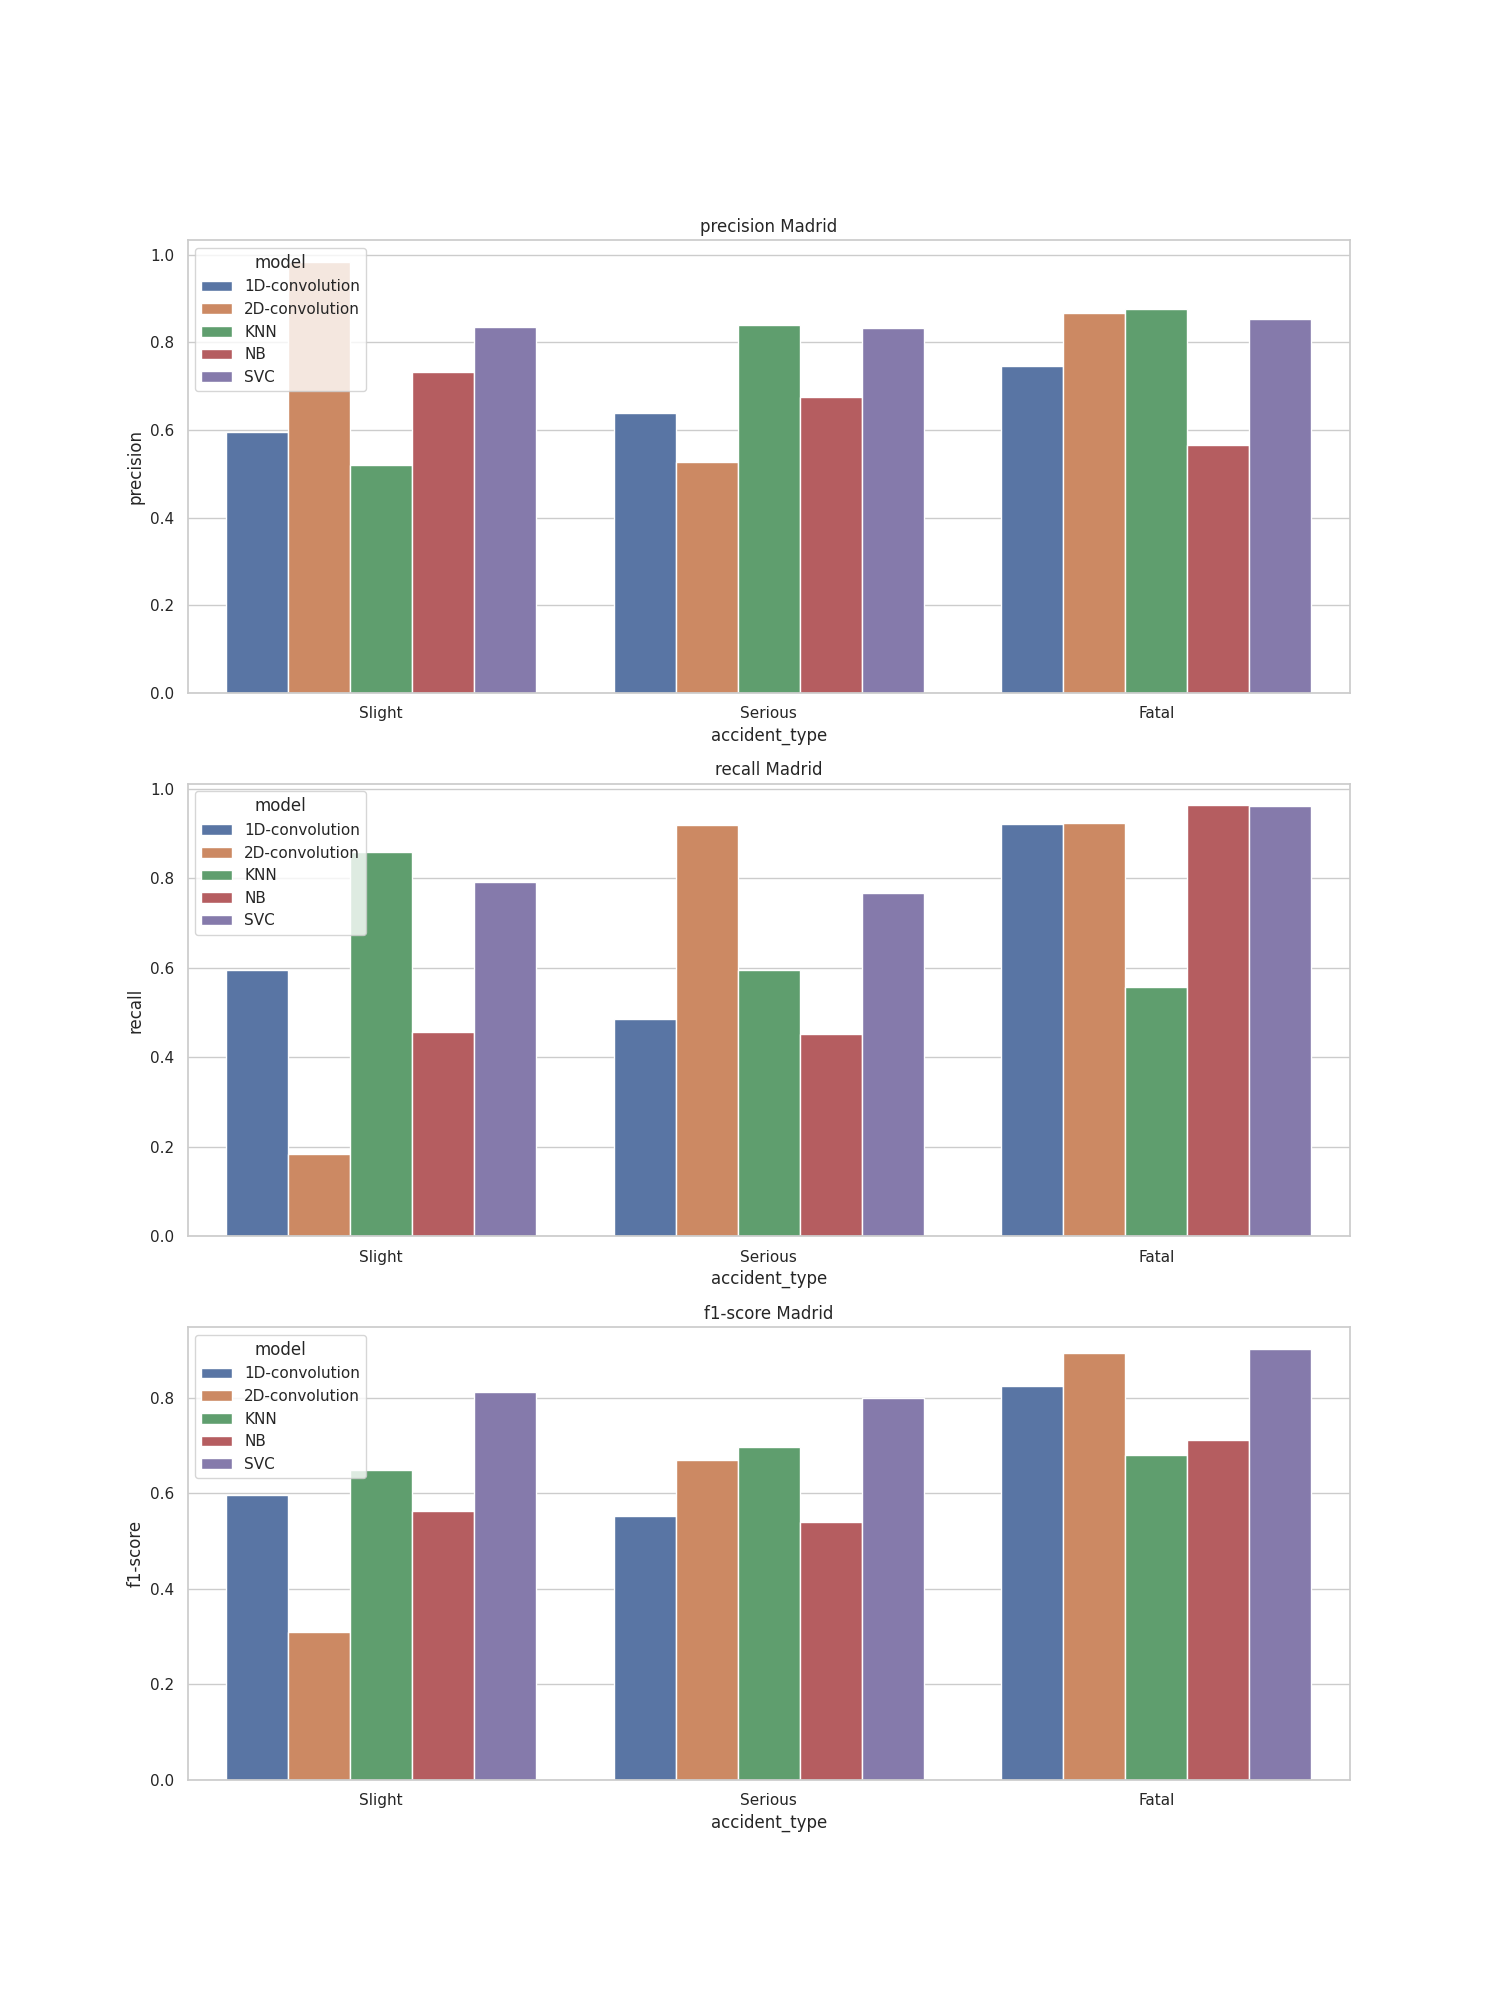
\includegraphics[width=13cm]{archivos/5.Resultados/ComparativaTrain}
      \caption{Comparativa de las métricas de las predicciones sobre el conjunto de entrenamiento de los modelos.}
      \label{ResultsTrainImage}
   \end{figure}



\subsection{Test}

  En esta subsección se discutirán los resultados comparativos sobre el conjunto de validación entre los cinco modelos entrenados. Esto es de vital importancia, ya que el objetivo de un modelo predictivo es la clasificación de datos futuros. Por lo tanto, comprobaremos su calidad mediante los datos de test.

  \subsubsection{Comparativa de reportes de clasificación}

    Al igual que en la comparativa de datos de entrenamiento, se muestran las métricas de clasificación resultantes en la tabla \eqref{TestClassificationReport} para cada una de las clases predecidas sobre el  conjunto de test. Estos reportes muestran la información con la que evaluaremos definitivamente los modelos, ya que explica cómo se comportan respecto a datos que nunca ha visto. Analizando el F1-score de los reportes se puede observar que el rendimiento de los modelos no se asemeja mucho a los resultados sobre el conjunto de entrenamiento. El modelo que mejor media F1-score presenta para las clases leves es la red convolucional de dos dimensiones \eqref{TestClassificationReport:CNN2D}, llegando a un \textit{0.949}, muy por encima del siguiente modelo \glsentryshort{knn} que ofrece un valor de \textit{0.81}. Además, la \glsentryshort{cnn2d} también ofrece la mejor métrica para los accidentes severos \textit{0.149}, llegando al doble de rendimiento respecto al modelo que le sigue, de nuevo el \glsentryshort{knn} con \textit{0.076}. En lo que respecta a los accidentes fatales, el modelo que mejor se adapta a esta clasificación es la red neuronal convolucional de una dimensión \eqref{TestClassificationReport:CNN1D}, obteniendo un \textit{0.004}, el doble que el \glsentryshort{knn} \eqref{TestClassificationReport:KNN}, que es de nuevo el siguiente mejor modelo en esta clase con \textit{0.002}.


    \begin{table}[H]
        \scriptsize
        \renewcommand{\arraystretch}{1.1}

        \begin{subtable}{.5\textwidth}     
          \csvautotabular{archivos/5.Resultados/CNN/1D/1DClassificationReportTest.csv}
          \caption{CNN-1D.}
          \label{TestClassificationReport:CNN1D}
        \end{subtable}
        \hspace{1em}
        \begin{subtable}{.5\textwidth}
          \csvautotabular{archivos/5.Resultados/NB/NBClassificationReportTest.csv}
          \caption{GNB.}
          \label{TestClassificationReport:GNB}
        \end{subtable}
        \vspace*{0.5 cm}
        \begin{subtable}{.5\textwidth}     
          \centering
          \csvautotabular{archivos/5.Resultados/SVC/SVCClassificationReportTest.csv}
          \caption{SVC.}
          \label{TestClassificationReport:SVC}
        \end{subtable}
        \hspace{1em}
        \begin{subtable}{.5\textwidth}     
          \csvautotabular{archivos/5.Resultados/KNN/KNNClassificationReportTest.csv}
          \caption{KNN.}
          \label{TestClassificationReport:KNN}
        \end{subtable}
        %\vspace*{0.5 cm}
        \begin{subtable}{1\textwidth}     
          \centering
          \csvautotabular{archivos/5.Resultados/CNN/2D/2DClassificationReportTest.csv}
          \caption{CNN-2D.}
          \label{TestClassificationReport:CNN2D}
        \end{subtable}

      \caption{Métricas clasificación para el conjunto de test.}
      \label{TestClassificationReport}
    \end{table}


  \subsubsection{Comparativa de matrices de confusión}

    En la figura \eqref{ConfusionMatrixTestImages} se muestran las matrices de confusión aplicadas al conjunto de test, se observa una representación visual de las métricas de clasificación. Esto permite atender a que los modelos \glsentryshort{gnb} \eqref{ConfusionMatrixTestImages:GNB}, \glsentryshort{svc} \eqref{ConfusionMatrixTestImages:SVC} y \glsentryshort{cnn2d} \eqref{ConfusionMatrixTestImages:2D} no clasifican correctamente ninguna de las observaciones de accidentes fatales, mientras que \glsentryshort{knn} \eqref{ConfusionMatrixTestImages:KNN} clasifica uno y \glsentryshort{cnn1d} \eqref{ConfusionMatrixTestImages:1D} clasifica cinco. En lo que respecta a los accidentes leves el modelo \glsentryshort{cnn2d} \eqref{ConfusionMatrixTestImages:2D} es el que mayor número clasifica correctamente, al igual que los accidentes serios. Esto se debe a la naturaleza de las redes aplicada a la complejidad del problema, cada una de ellas encuentra patrones diferentes dependiendo de los mapas de características resultantes de las convoluciones de cada red.

    \begin{figure}[H]
        \centering
        \begin{subfigure}{0.4\textwidth}
            \includesvg[scale=0.35]{archivos/5.Resultados/CNN/1D/1DConfusionMatrixTest}
            \caption{CNN-1D.}
            \label{ConfusionMatrixTestImages:1D}
        \end{subfigure}
        \hspace{3em}
        % Añadir el espacio deseado, si se deja la linea en blanco la siguiente subfigura ira en una nueva linea
        \begin{subfigure}[b]{0.4\textwidth}
            \includesvg[scale=0.35]{archivos/5.Resultados/CNN/2D/2DConfusionMatrixTest}
            \caption{CNN-2D.} 
            \label{ConfusionMatrixTestImages:2D}
        \end{subfigure}
        \vspace*{0.5 cm}
        \begin{subfigure}[b]{0.4\textwidth}
            \includesvg[scale=0.35]{archivos/5.Resultados/NB/NBConfusionMatrixTest}
            \caption{GNB.}
            \label{ConfusionMatrixTestImages:GNB}
        \end{subfigure}
        \hspace{3em}
        \begin{subfigure}[b]{0.4\textwidth}
            \includesvg[scale=0.35]{archivos/5.Resultados/KNN/KNNConfusionMatrixTest}
            \caption{KNN.}
            \label{ConfusionMatrixTestImages:KNN}
        \end{subfigure}
        %\vspace*{0.5 cm}

        \begin{subfigure}[b]{0.4\textwidth}
            \includesvg[scale=0.35]{archivos/5.Resultados/SVC/SVCConfusionMatrixTest}
            \caption{SVC.}
            \label{ConfusionMatrixTestImages:SVC}
        \end{subfigure}

        \caption{Matrices de confusión de los modelos sobre el conjunto de test.}
        \label{ConfusionMatrixTestImages}
     \end{figure}

  \subsubsection{Comparativa entre modelos}

    A continuación se puede observar una representación visual \eqref{ResultsTestImage} de las métricas analizadas en el apartado anterior, donde se muestra la precisión, exhaustividad y f1-score para cada modelo respecto al conjunto de datos de test.

    \begin{figure}[H]
        \centering
        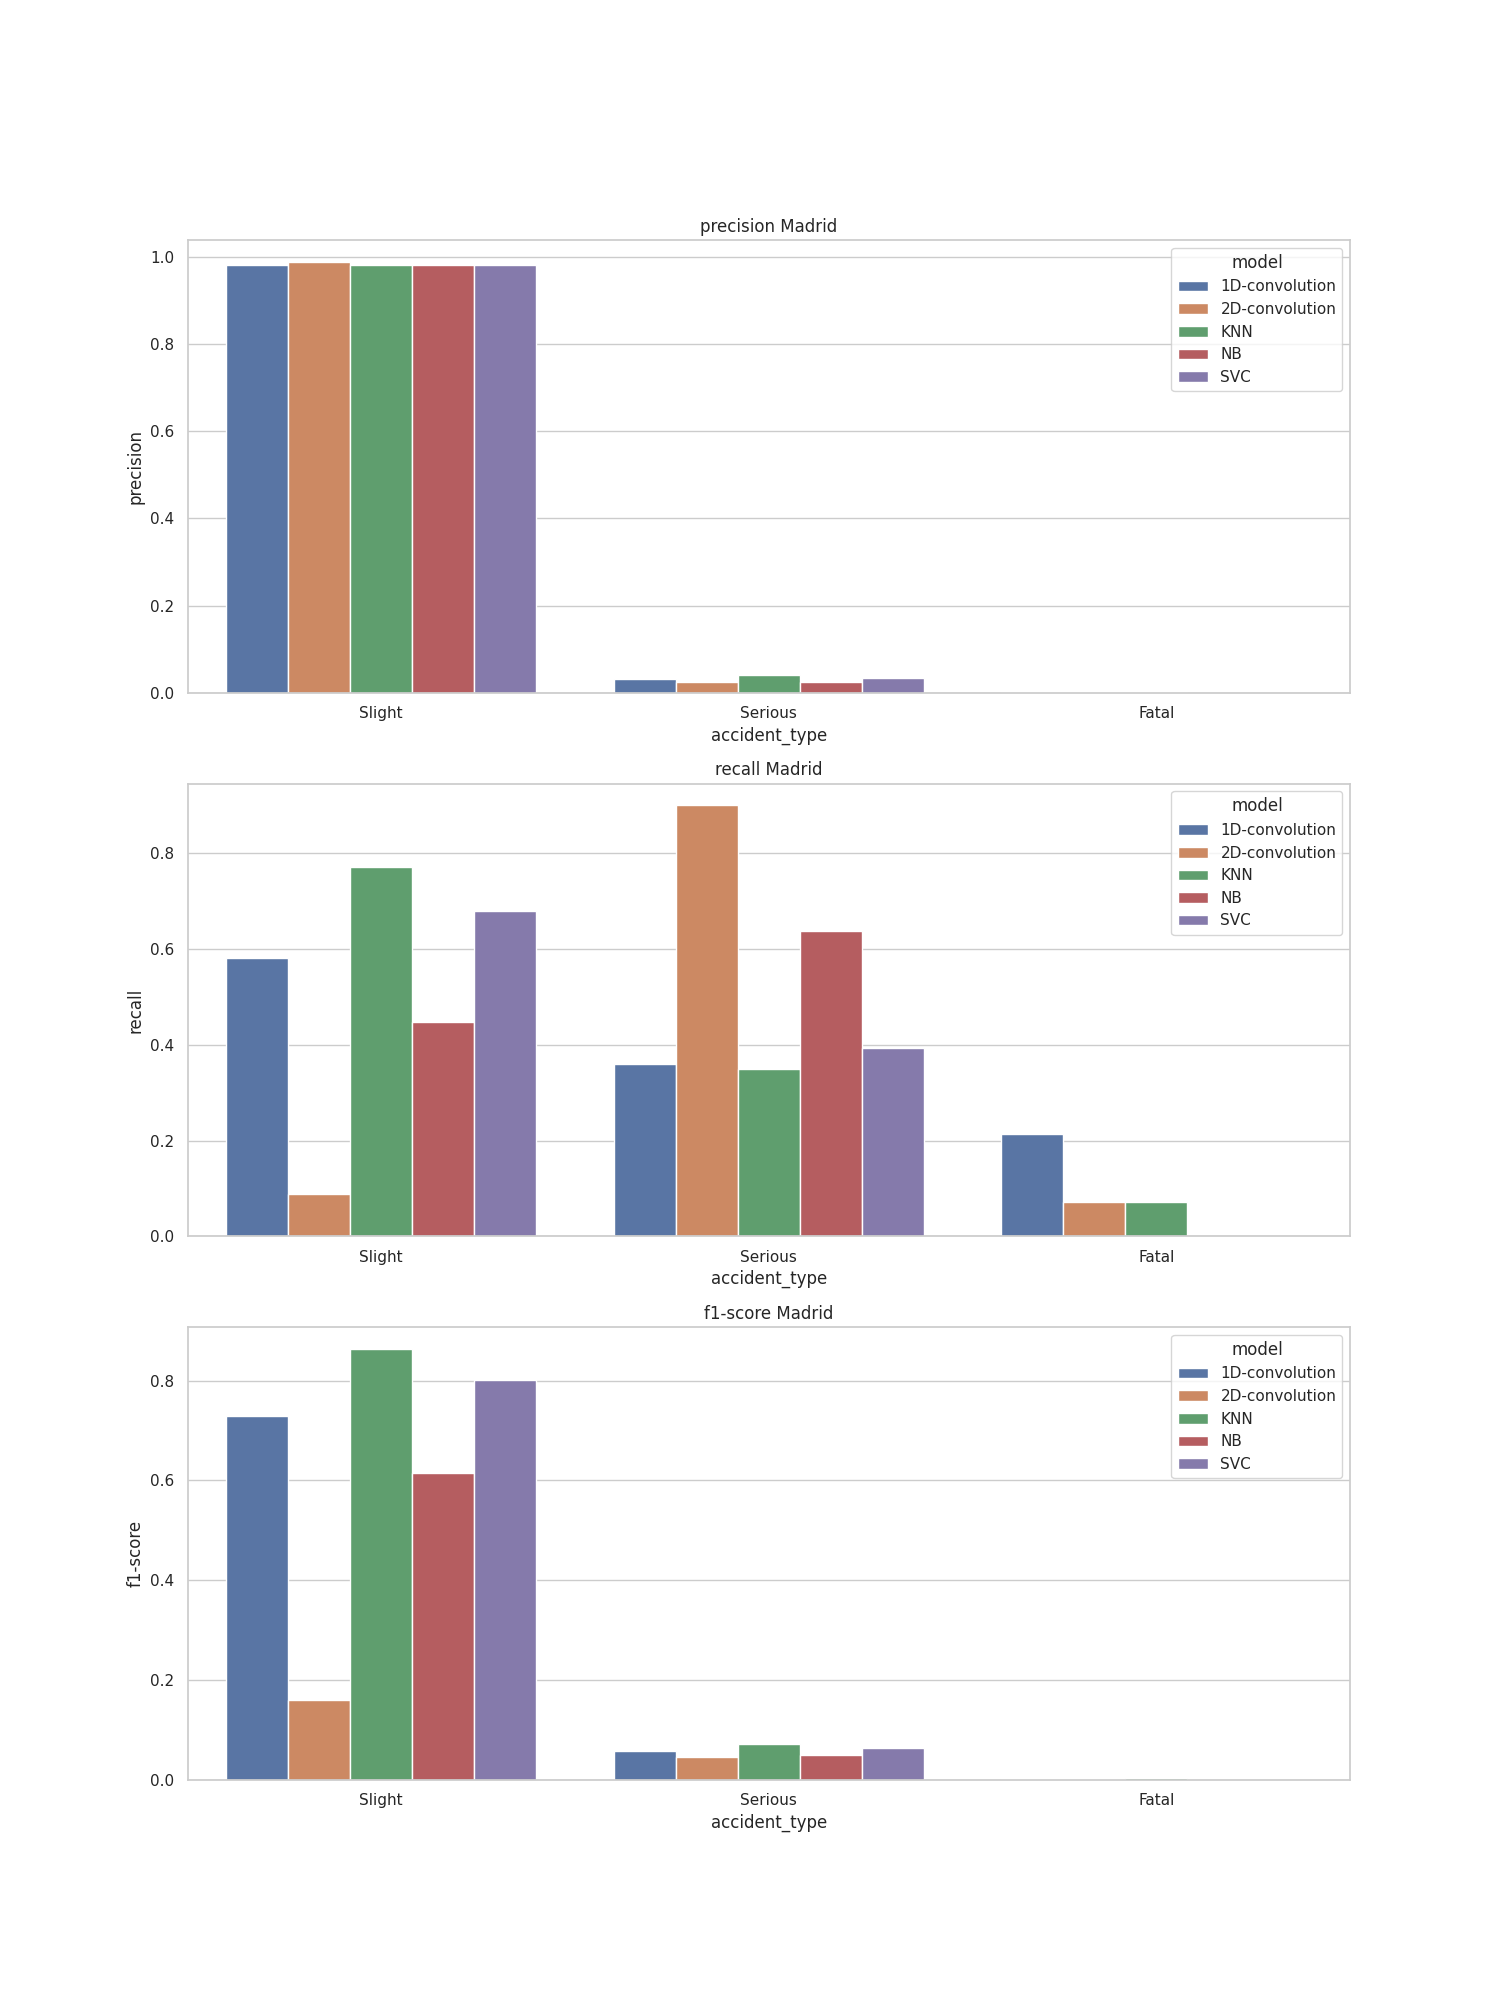
\includegraphics[width=13cm]{archivos/5.Resultados/ComparativaTest}
        \caption{Comparativa de las métricas de las predicciones sobre el conjunto de test de los modelos.}
        \label{ResultsTestImage}
     \end{figure}

    Como se puede comprobar en los resultados de los experimentos, las dos arquitecturas convolucionales propuestas superan en rendimiento al resto de modelos de referencia para cada una de las clases de accidentes (leve, severo y fatal). La ventaja de disponer de estas dos nuevas arquitecturas es que cada una de ellas funciona mejor dependiendo del tipo de clase a predecir. Esto permite diseñar un sistema Ensemble en el que se utilicen las dos redes entrenadas para combinar sus resultados, de tal forma que se utilizaría la red \glsentryshort{cnn1d} para predecir accidentes de carácter leve y fatal mientras que la red \glsentryshort{cnn2d} clasificaría los accidentes serios.